\documentclass[a4paper, 12pt]{article}
\usepackage[utf8]{inputenc}
\usepackage[brazil]{babel}
\usepackage[lmargin=2cm, tmargin=3cm,rmargin=2cm,bmargin=2cm]{geometry}
\usepackage[T1]{fontenc}
\usepackage{blindtext}
\usepackage{setspace}
\usepackage{multirow}
\usepackage{fancyhdr}
\usepackage{parskip}
\usepackage{graphicx}
\usepackage{subfig}
\usepackage{url}
\usepackage{natbib} 
\usepackage{booktabs}

\bibliographystyle{acm}





\begin{document}




\thispagestyle{empty}
    \begin{center}
        
        
\includegraphics[scale=0.1]{Brasão_ufra.png}\\
        \vspace{0.25cm}
        \textbf{UNIVERSIDADE FEDERAL RURAL DA AMAZÔNIA}\\
        \textbf{PRÓ-REITORIA DE PESQUISA E DESENVOLVIMENTO TECNOLÓGICO}\\
        \textbf{PROGRAMA DE INICIAÇÃO CIENTÍFICA E TECNOLÓGICA}\\
        \vspace{2cm}
         \textbf{Orientador \\ GILBERTO NERINO DE SOUZA JUNIOR}\\
        \vspace{0.5cm}
        \textbf{Discente \\ MIKEIAS DOS SANTOS OLIVEIRA}\\
        \vspace{1cm}
        RELATÓRIO PARCIAL REFERENTE AO CICLO PROGRIDI 2022/2023\\
        \vspace{2cm}
        \textbf{PROJEÇÕES DE TENDÊNCIAS RELACIONADAS AS ATIVIDADES AGROPECUÁRIAS ATRAVÉS DE TÉCNICAS DE MINERAÇÃO DE DADOS E INTELIGÊNCIA ARTIFICIAL NO ESTADO DO PARÁ}\\
        \vspace{2cm}
        \\
        \\
        \vspace{2cm}
        \textbf{Paragominas/PA}
        \textbf{2023}\\
        \vspace{1.5cm}
  
    \end{center}


\newpage




\pagestyle{fancy}
\fancyhf{}

\fancyhf[OHC]{\textbf{Projeções de tendências relacionadas as atividades agropecuárias através de técnicas de mineração de dados e inteligência artificial para o estado do Pará}}

\vspace{2cm}
\begin{center}
   
   Projeções de tendências relacionadas as atividades agropecuárias através de técnicas de mineração de dados e inteligência artificial para o estado do Pará
\end{center}

\tableofcontents
\newpage


\section{Introdução}


Muitas das políticas agrícolas para a Amazônia brasileira tiveram implantações no Estado do Pará, seja pelas condições edafoclimáticas, seja pelas condições logísticas que tornaram o território paraense parte fundamental da fronteira agrícola brasileira \cite{maeda2009predicting}. O Pará detém algumas trajetórias produtivas de destaque na agropecuária brasileira \cite{pespectiva}, a exemplo da produção de açaí, abacaxi, cacau, mandioca e dendê, as quais são as principais do Brasil; no que se refere a pecuária, o Pará é o quarto em rebanho de bovinos e equinos, e o primeiro no de búfalos (IBGE, 2021).

Convêm destacar que as atividades rurais detêm efeitos a jusante e a montante da cadeia produtiva, isto é, incorporam elementos fornecedores de insumos e intermediários dos bens finais \cite{pinage2022forest}. Além de propiciar um ambiente de negócios crescente e dinâmico, em especial, quando se considera a geração de empregos e a criação de empresas no ramo agropecuário, inclusive formais, que colaboram tanto na arrecadação de impostos, quanto no desempenho econômico estadual e do país (BRASIL, 2021).

O espectro econômico da produção agropecuária é conhecido, visto que a lógica de mercado tende a seguir sequências lineares de encadeamento de fatores produtivos (capital, trabalho e uso da terra) e dos setores econômicos (primário, secundário e terciário). Assim, enquanto um ramo produtivo é ativado ou incrementado, a resposta é um aumento da demanda dos fatores de produção e de elevação do uso de outros segmentos da economia. Aspectos de ordem institucional moldam o mercado de commodities amazônicas \cite{bolch2020remote}. A maioria das questões institucionais estão ligadas à contenção do desmatamento, com foco na sustentabilidade e na proteção das áreas florestadas. O intuito é estabelecer um conjunto de incentivos e desincentivos capazes de influenciar de maneira direta na redução da degradação ambiental ligada ao agronegócio e migrar para uma economia de base sustentável \cite{zambon2019revolutionizing}. Nesse sentido, as investigações pretendidas são direcionadas para além das forças de mercado (demanda e oferta), dessa forma chegando às ações estatais, através de políticas públicas e capacidade de coerção, que em tese, possuem capacidade de influenciar a trajetória produtiva e no uso da terra, expressa ao longo do tempo nas quantidades produzidas, exportadas, e na criação de empresas e empregos.

Neste contexto, novas tecnologias têm se destacado nos mercados produtivos, em especial, no agronegócio. Tudo para facilitar a gestão, com o objetivo de diminuir o tempo e o custo, e aumentar a produtividade e a sustentabilidade \cite{renzcherchen2021desenvolvimento}. São desde aplicativos para promover a previsibilidade climática e classificação do uso da terra com base em imagens de satélites e drones, desde softwares de gerenciamento das atividades da fazenda, a sistemas de acompanhamento das oscilações de preços do mercado \cite{gardon2020brazil}.

Atualmente, as tecnologias de Inteligência Artificial atuam em uma grande quantidade de dados, fornecendo diagnósticos e previsibilidade, projetando cenários, antecipando situações indesejáveis e fazendo recomendações em tempo real. Em consonância, o uso da geo informação, ciência de dados e análise de séries temporais também são ferramentas que permitem aprofundar o conhecimento e estabelecer relações entre as mais diversas variáveis. Ajudam essencialmente a compreender as dimensões espaciais e temporais dos dados, ao nível de identificar quais dados devem ser coletados, com que frequência e em quais áreas determinadas \cite{de2020mineraccao}.

Em contrapartida, nem todos os dados desejados estão disponíveis, e mesmo se existirem, muitas vezes, deverão ser remodelados até alcançarem um grau de relevância satisfatório. Paralelamente, existe uma infinidade de técnicas que podem contribuir com a projeção de séries temporais e o entendimento histórico dos dados. Além disso, base de dados públicas raramente encontram-se organizadas, sem qualquer integração, o que dificulta o uso de certos algoritmos de modo a gerar dados confiáveis e mais relevantes para o tomador de decisão, seja público ou privado. Assim, o estudo desses dados e técnicas avançadas se torna fundamental para o planejamento e a definição de estratégias, seja para aproveitar o desempenho produtivo do setor agropecuário, com o atendimento da demanda de mão-de-obra ou oferta de produtos e serviços, seja para conter alguma
externalidade, como a degradação ambiental.


\section{Material e métodos}

\subsection{Fonte de dados}
As pesquisas usarão de fontes de dados públicas para a criação de banco de dados para análise das variáveis e relacioná-las sob a perspectiva
econômica, social e ambiental, a saber: IBGE (Instituto Brasileiro de Geografia e Estatística), SIDRA-IBGE (Sistema IBGE de Recuperação Automática), Mapbiomas Brasil.

\subsection{Processamento de dados}

O processamento dos dados e análise ocorreram na plataforma de mineração de dados Orange, através da linguagem de programação Python e suas
bibliotecas de aprendizado de máquina e ciência de dados, e na plataforma gratuita Google Earth Engine para a investigação de imagens de satélite.
Buscar-se-a dados públicos com o objetivo de predizer as tendências de crescimento, estabilização ou redução, a saber: em hectares, Floresta,
Pastagem, Soja, Lavouras Temporárias (junção de milho, mandioca, arroz e abacaxi e outras lavouras temporárias); em valores quantitativos,
Estabelecimentos agropecuários e Empregos agropecuários. Os dados coletados serão dados anuais, num intervalo entre 1985 e 2020, somando 36 anos
de análise.

Inicialmente será necessário tratar e integrar os dados das diferentes bases formando um conjunto de dados únicos. Posteriormente serão criadas
instâncias intermediárias formando um novo conjunto de dados com base semestral, em vez de anual, visando aumentar a quantidade de dados para 72 instâncias com a criação dos registros sintéticos. Após a implementação da nova estrutura de dados, técnicas de interpolação linear, que imputam valores ausentes espaçados e lineares entre os dois pontos de dados poderão ser utilizados com a finalidade de tratar os registros faltantes na tentativa de obtenção da menor taxa de perca de informação possível.

Os métodos explorados para realizar a projeção serão: ARIMA (modelo estatístico), BlockRNNModel, LSTM, GRU, NBEATSModel, TCNModel,
TransformerModel (modelos baseados em redes neurais artificiais e deep learning) e modelos linha de base (modelos ingénuos). É importante ressaltar que apesar da utilização de modelos baseados em aprendizado profundo, é esperado que esses modelos apresentem um desempenho inferior ao que seria esperado, visto que a quantidade de dados disponíveis são insuficientes para justificar um possível bom desempenho do modelo, entendendo que esse comportamento só poderia ser explicado pelo aprendizado por chance, (boa acurácia do modelo por chance aleatória estatística) implicando que o resultado não necessariamente signifique uma boa generalização do modelo. 

Para a escolha dos parâmetros dos modelos utilizar-se-á inicialmente o algorítimo RandomSearch para definir quais os intervalos de parâmetros pode ser encontrado um ótimo local e após isso será feita a utilização do também algoritmo de otimização, GridSearch, para aprofundar a análise do ótimo local com o intuito de otimizar ainda mais o modelo. A implementação do método de otimização descrito foi desenhado considerando que o RandomSearch apresenta um desempenho maior porém não aprofunda todas as combinações possíveis de hiper-parâmetros, enquanto o GridSearch apresenta um custo computacional exponencialmente maior ao decorrer que a área de parâmetros aumenta, mas em compensação irá avaliar todas as combinações possíveis. O processo de otimização que será considerado tenta equilibrar os trade-off ao mesmo tempo que tenta explorar a vantagem de utilização de cada algoritmo. A mensuração do desempenho do modelo em face a aplicação de técnicas de otimização deve ser através de validação cruzada, dado que a otimização pode implicar no sobre-ajuste dos dados de teste, significando uma má generalização do modelo.

% --------------------

% --------------------
\subsubsection{Dados de cobertura da terra}

O MapBiomas é uma iniciativa sem fins lucrativos do Sistema de Estimativas de Emissões de Gases de Efeito Estufa do Observatório do Clima mantido e desenvolvido por várias instituições, entre elas, ONGs e Universidades Federais. Seus dados são disponibilizados na plataforma gratuitamente que também disponibiliza tutoriais para baixar os arquivos. 

A sua utilização no presente projeto se dá pela possibilidade de adquirição dos dados de forma mais atualizada, veloz e segundo os próprios integrantes do projeto, mais barata, em comparação com outros métodos que almejam a mesma finalidade. Os dados de cobertura de terra do MapBiomas foram extraídos em sua totalidade, entretanto, para finalidade de alinhamento das informações dispostas com o objetivo do projeto, os dados foram filtrados para incluir somente os registros do estado do Pará. 

Após a limpeza, foi contabilizado registros de 143 diferentes municípios do estado do Pará. Um dos atributos disponibilizados na base é referente ao bioma, entretanto, por se limitar apenas a duas categorias distintas, foi desconsiderada. As informações preservadas se reservaram ao município, identificador de classe, nome da classe e ano do registro. As classes de interesse foram mantidas e as demais foram descartadas, sendo classes de interesse: Formação florestal, pastagem, grãos de soja, outras lavouras temporárias e outras lavouras permanentes. Os dados foram então armazenados e reservados para uma posterior integração com os demais dados.

\subsubsection{Dados do IBGE}

% O que
A SIDRA é um banco de dados agregados que disponibiliza séries temporais de diversas áreas, como: Administração pública, agroindústria, economia, economia agrícola e estatística. As tabelas extraídas foram: Área plantada, área colhida, quantidade produzida, rendimento médio e valor da produção das lavouras temporárias; Área plantada, área colhida, quantidade produzida, rendimento médio e valor da produção das lavouras permanentes; Quantidade produzida e valor da produção na silvicultura, por tipo de produto da silvicultura; Efetivo dos rebanhos, por tipo de rebanho. 
% Por que?
O Sistema IBGE De Recuperação Automática é uma ferramenta que possibilita a recuperação de dados diretamente do banco de dados do IBGE. Dentro do sistema, diversas tabelas são disponibilizadas com as mais diferentes finalidades. Sua maior relevância para o projeto é em virtude da confiabilidade dos dados, considerando que, são fornecidos diretamente pelo maior órgão oficial de estatística do Brasil.
% Como?
Os dados podem ser adquiridos através de API. Os registros possuíam algumas características que ocasionariam erros, visto isso, os dados passaram por transformações e limpezas que garantiram a qualidade e coerência dos dados. Após essa limpeza, as informações foram mescladas com os dados de cobertura da terra e realizado uma cuidadosa análise. 

\subsection{Projeções e interpretação dos dados gerados}

Após encontrar os melhores conjuntos de parâmetros para um determinado alvo, executar-se-á os modelos que tiveram melhor desempenho gerando
projeções, que no que lhe concerne, podem servir de base para gerar os gráficos e análise de tendências para cada um dos alvos determinados.
Os gráficos serão validados por especialistas e interpretados pela equipe do projeto com foco em uma visão das tendências de crescimento, queda ou
estabilização, que por sua vez formarão os relatórios técnicos do framework. Visando o aprofundamento das análise, foi também utilizado os dados, referentes as regiões geográficas e seus detalhamentos como, regiões intermediárias e imediatas, conforme é adotado pelo IBGE desde 2017. 



\section{Resultados parciais}

As análise preliminares tiveram um caráter mais exploratório, ou seja, o enfoque foi analisar se os dados dispostos disponham de padrões e tendências esperadas. Dos anos de 1985 até 2021, notou-se uma tendência de crescimento de produção pecuária no estado do Pará, em decorrência disso, é esperado que exista uma correlação entre a área de pastagem e o número de rebanhos. Para podermos confirmar a hipótese, foi gerado um gráfico de correlação de Pearson, que obteve os seguintes resultados: 

\begin{figure}[hbt!]
    \centering
    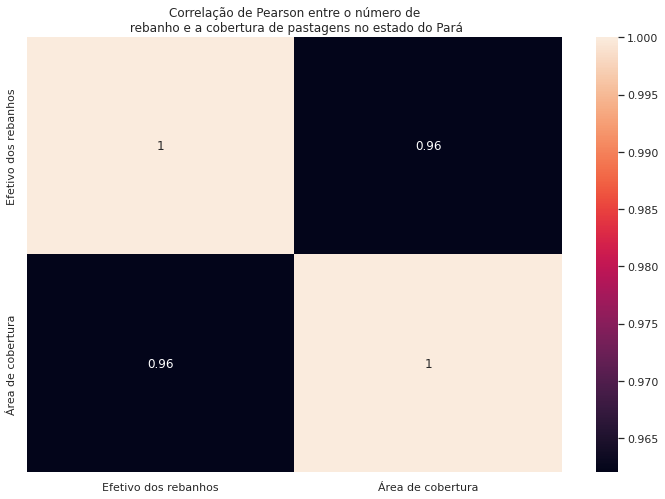
\includegraphics[width=0.7\columnwidth]{src/corr_rebanho_pastagem.png}
    \caption{Correlação entre o número de cabeças de rebanhos em relação a área de cobertura de pastagem no estado do Pará}
    \label{fig:corr_rebanho_pastagem}
\end{figure}

As duas variáveis demonstraram uma alta correlação positiva, o que significa que o crescimento de uma está associada positivamente ao crescimento da outra. Para aprofundar a análise, foi gerado também um gráfico que visa entender o comportamento dos dados ao decorrer dos anos e identificar anomalias e correlações entre eles.
\newpage
\begin{figure}[hbt!]
    \centering
    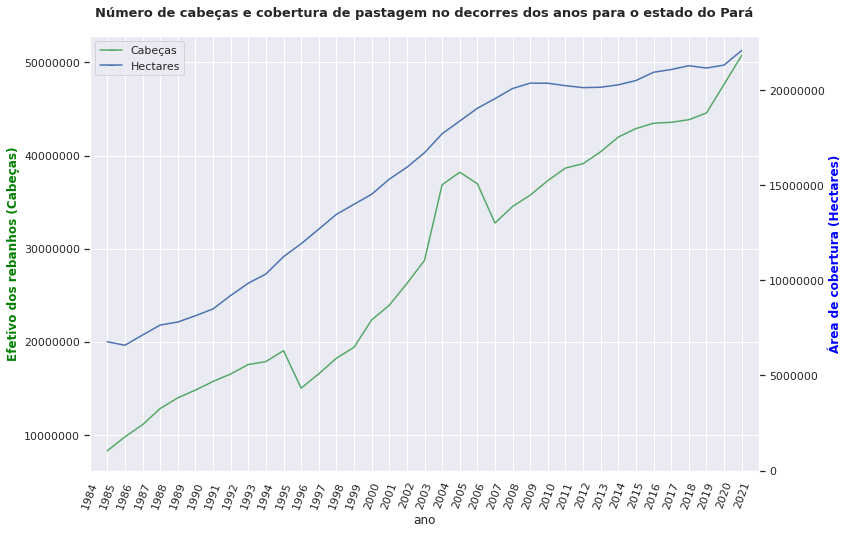
\includegraphics[width=0.9\columnwidth]{src/numero-cabecas-cobertura-pastagem.png}
    \caption{Gráfico temporal de número de cabeças de rebanhos e área de cobertura de pastagem no estado do Pará}
    \label{fig:numero_cabecas_cobertura_pastagem}
\end{figure}

\subsection{Dicionário de dados}
\thispagestyle{empty}

\subsection*{Apoio}
Esse projeto é um apoio da Universidade Federal Rural da Amazônia via edital PROIC/PIBITI.


\bibliography{obras}





\end{document}
